\documentclass{article} % For LaTeX2e
\usepackage{nips15submit_e,times}
\usepackage{hyperref}
\usepackage{url}
\usepackage{graphicx}
\usepackage{array}
\usepackage{afterpage}
%\documentstyle[nips14submit_09,times,art10]{article} % For LaTeX 2.09

\title{EEG curiosities -- follow-up}

\author{
Manuel Nickel
\\
%Technische Universit\"at M\"unchen\\
%Pittsburgh, PA 15213 \\
\texttt{manuel.nickel@tum.de} \\
\And
Dominik Irimi \\
%Affiliation \\
%Address \\
\texttt{dominik.irimi@gmail.com} \\
\AND
Christoph Dehner \\
%Affiliation \\
%Address \\
\texttt{dehner@in.tum.de} \\
\And
Roman C.~Podolski \\
%Affiliation \\
%Address \\
\texttt{roman.podolski@tum.de} \\
\And
Philipp Bergmann \\
%Affiliation \\
%Address \\
\texttt{philipp.bergmann@tum.de} \\
}

% The \author macro works with any number of authors. There are two commands
% used to separate the names and addresses of multiple authors: \And and \AND.
%
% Using \And between authors leaves it to \LaTeX{} to determine where to break
% the lines. Using \AND forces a linebreak at that point. So, if \LaTeX{}
% puts 3 of 4 authors names on the first line, and the last on the second
% line, try using \AND instead of \And before the third author name.

\newcommand{\fix}{\marginpar{FIX}}
\newcommand{\new}{\marginpar{NEW}}

\nipsfinalcopy % Uncomment for camera-ready version

\begin{document}


\maketitle

\begin{abstract}
To further examine the results presented in \emph{EEG curiosities} the EEG data was normalized and then visualized using t-SNE as well as trained on a neural net once again. Furthermore, data of several other participants and series has been tested in the same manner.
\end{abstract}

\section{Revisiting \emph{Participant 1, Series 1}}
The EEG dataset of \emph{Participant 1, Series 1} was normalized to a range of values between $-1$ and $+1$. Then another t-SNE plot was created to determine if this had any effect. Figure \ref{fig:eegP1S1} shows the result and no obvious difference compared to the previous runs without normalization.

\begin{figure}[h]
	\centering
	\hspace*{-1.7cm}
	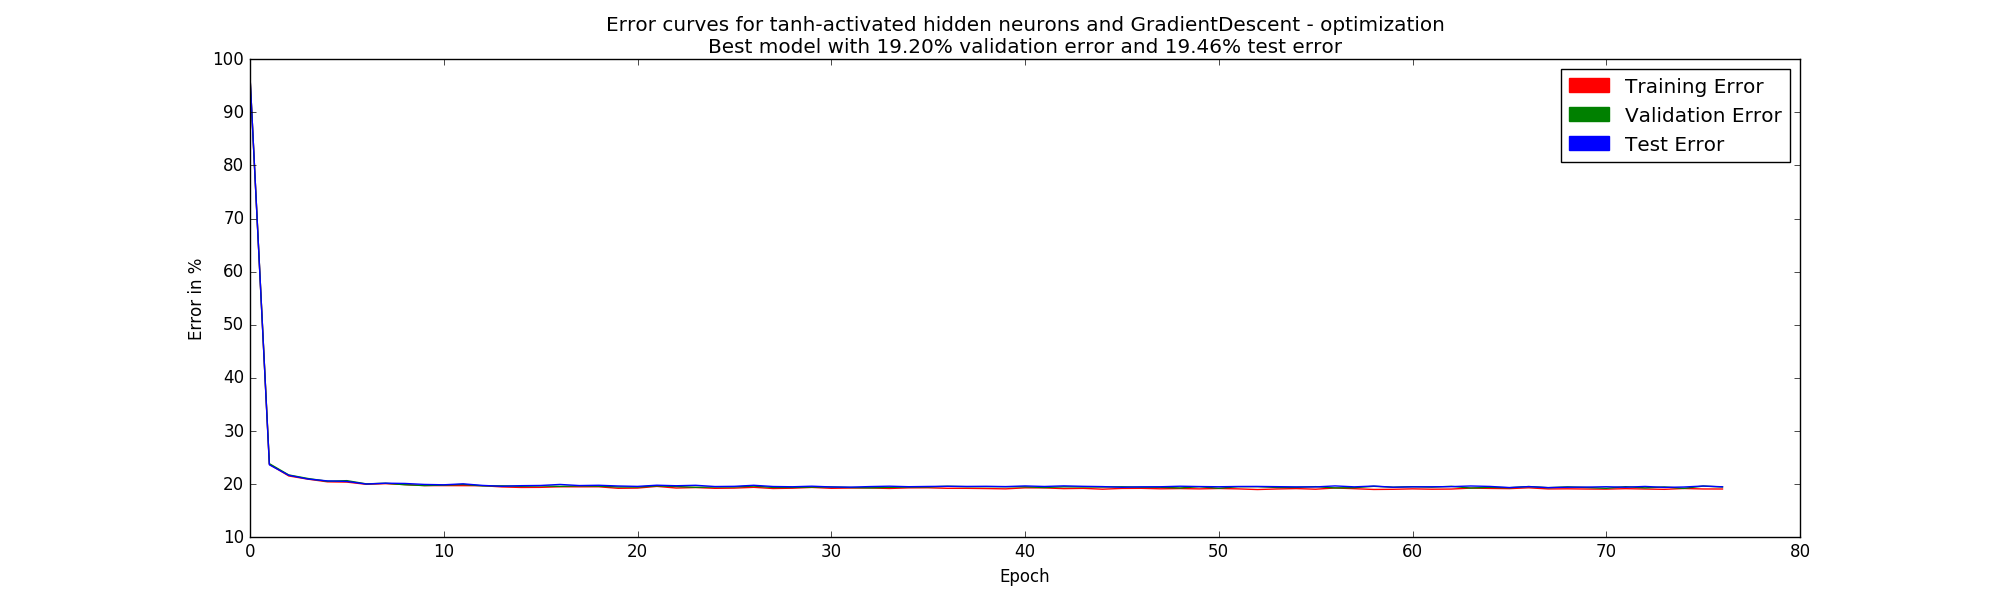
\includegraphics[width=1.25\textwidth]{eegnnP1S1.png}
	\caption{Classifying participant 1, series 1 trials using a feedforward neural net}
	\label{fig:eegnnP1S1}
\end{figure}

\begin{figure}[h]
	\centering
	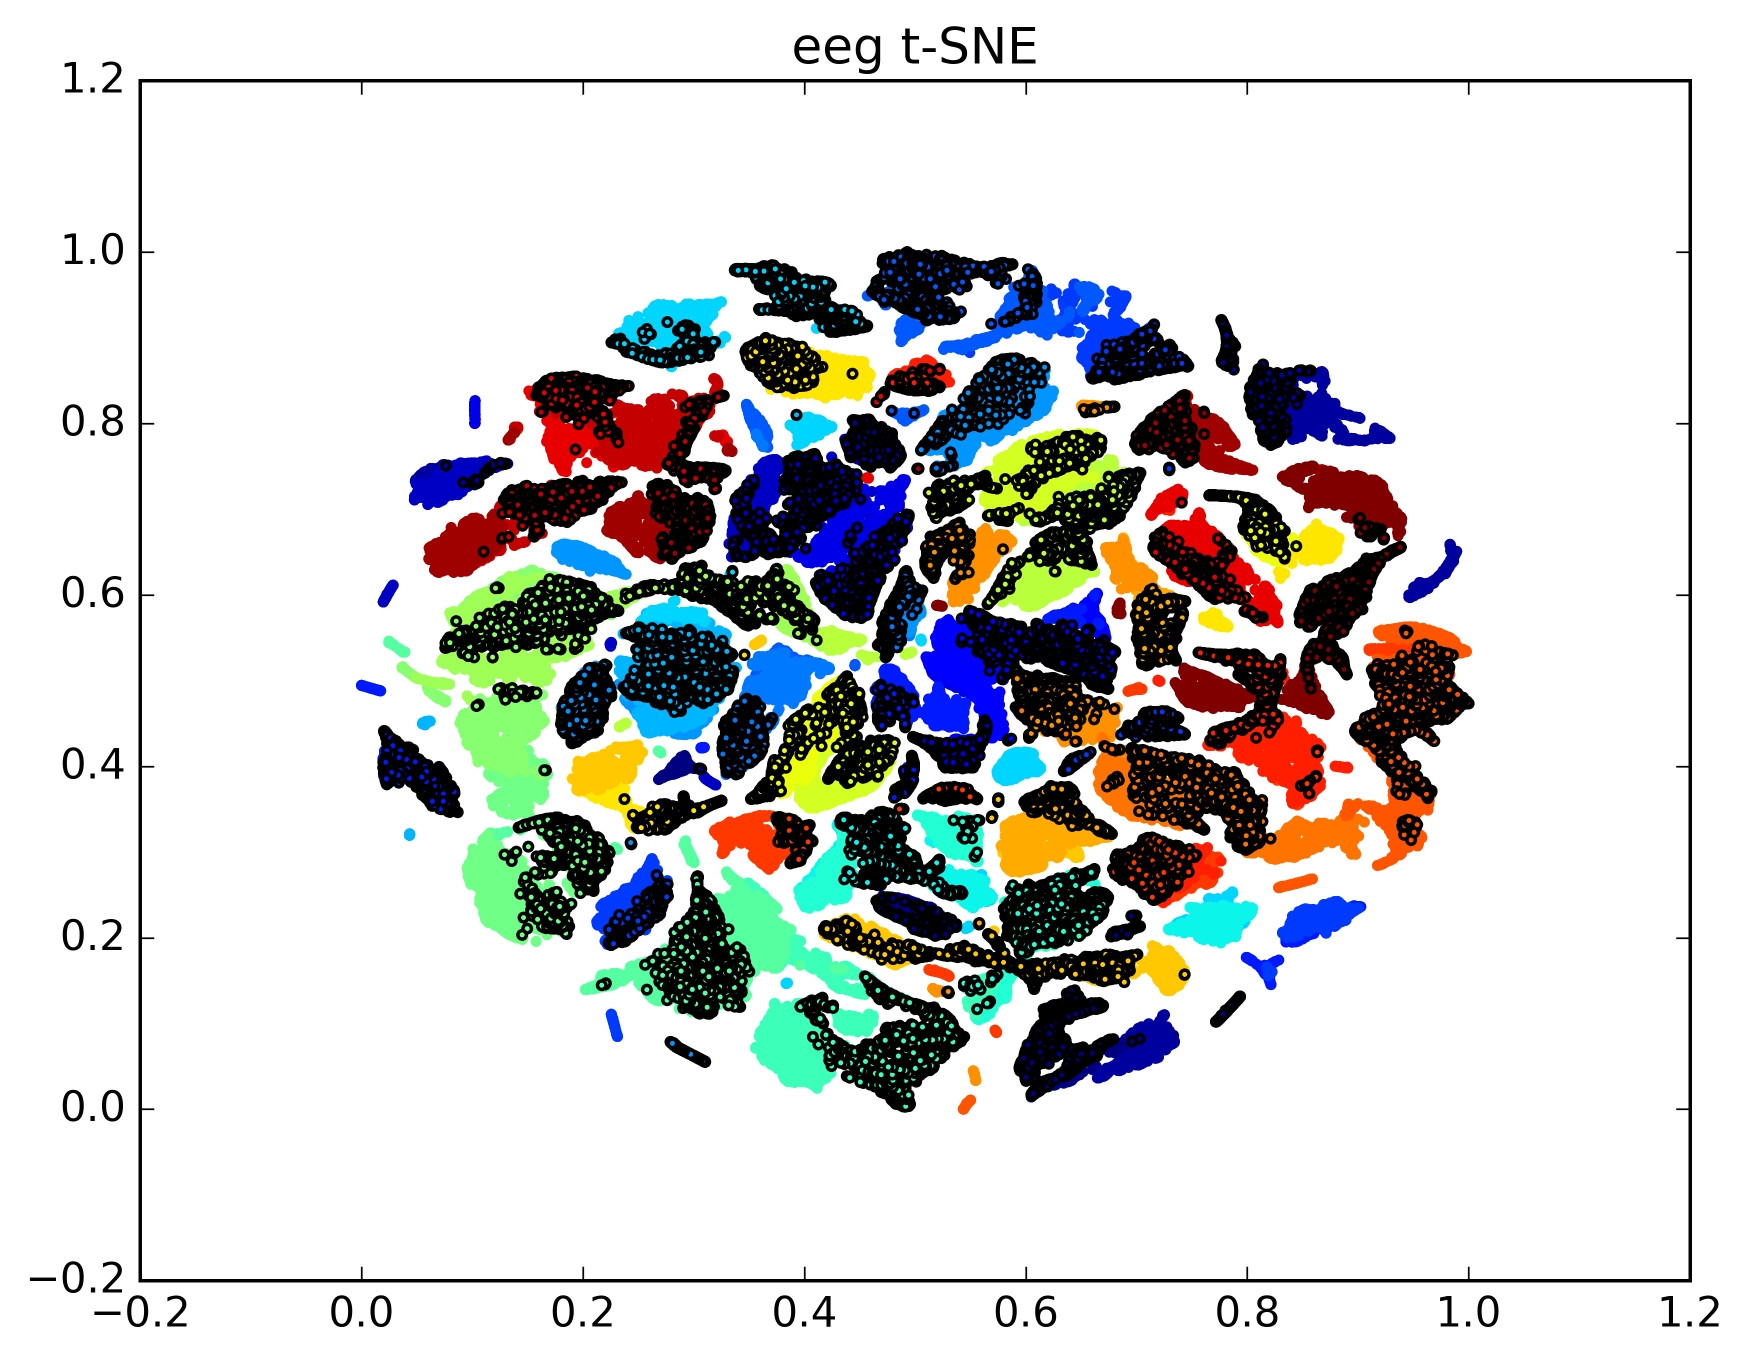
\includegraphics[width=1.0\textwidth]{eegP1S1.jpg}
	\caption{t-SNE plot for normalized participant 1, series 1 EEG data}
	\label{fig:eegP1S1}
\end{figure}

The now normalized data was also run through a feedforward neural net, trying to classify the various trials. Using the following settings, an error on the validation set of $19.20\%$ and en error on the test set of $19.46\%$ was achieved, which is a slight improvement over the best run without normalization:
\begin{itemize}
	\item Hidden Layer: 1
	\item Input neurons: 32
	\item Hidden neurons: 300
	\item Output neurons: 34
	\item Activation function: tanh
	\item Optimizer: Gradient Descent
\end{itemize}

A plot of the resulting error rates is shown in figure \ref{fig:eegnnP1S1}




\section{Analyzing data of other participants and series}
A random selection of datasets of other participants and series was chosen and the same procedure as before was applied to them. That is, for each dataset a t-SNE plot as well as a neural net run was performed. In the following the t-SNE plot and neural net results for \emph{Participant 1, Series 1} will be used as a reference, the new tests will be compared to. One may have to emphasize, the very extreme error rates noted in the table are NO typos. The results are shown and briefly discussed in table \ref{tbl:tests}. The images were cropped down for better readability. Bigger versions are attached as separate files.

\begin{figure}
	\centering
	\begin{tabular}{|m{3cm}|m{2.2cm}|m{1cm}|m{8cm}|}
		\hline  \textbf{t-SNE plot} & \textbf{Dataset} & \textbf{Test error} & \textbf{Comment} \\ 
		\hline \rule{0pt}{15ex}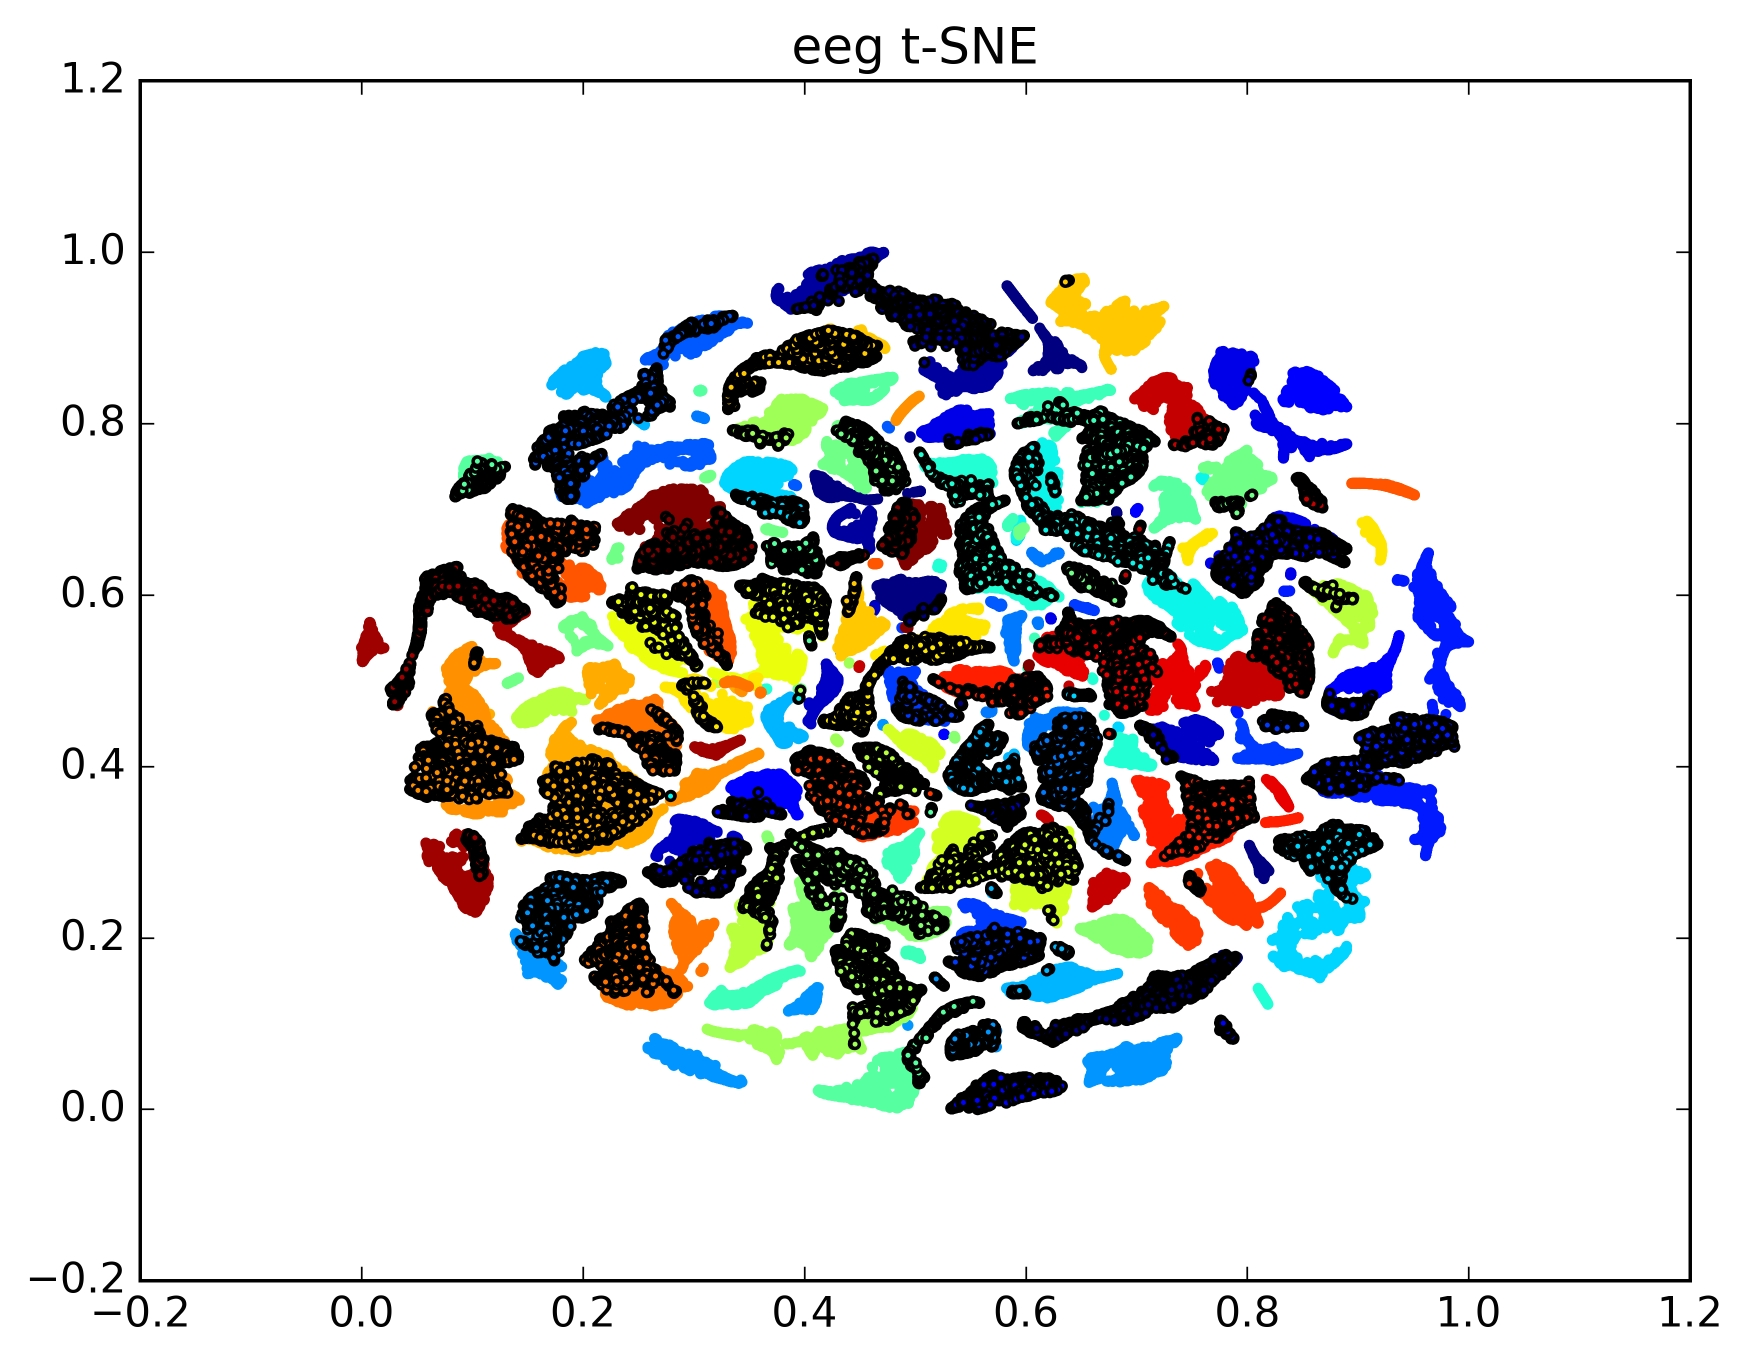
\includegraphics[width=3cm]{eegP1S2.jpg} & Participant 1, Series 2 & $0.08\%$ & In the t-SNE plot the data is even better separated. The neural net can perfectly classify the trials ($0.08\%$ is not a typo)\\ 
		\hline \rule{0pt}{15ex}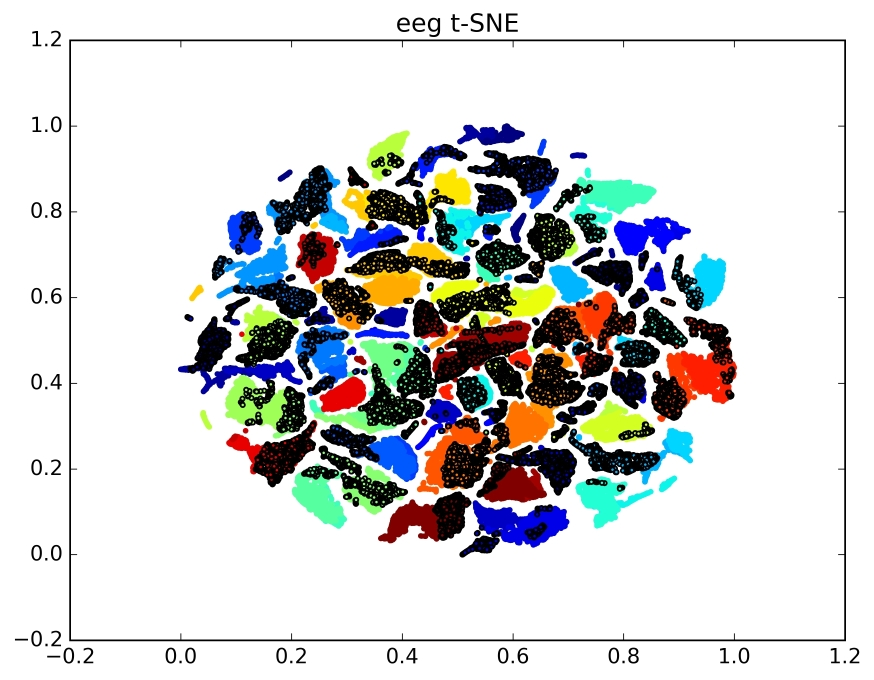
\includegraphics[width=3cm]{eegP4S9.jpg} & Participant 4, Series 9 & $16.75\%$ & Not as well separated data with correspondingly worse performance on the neural net. \\ 
		\hline \rule{0pt}{15ex}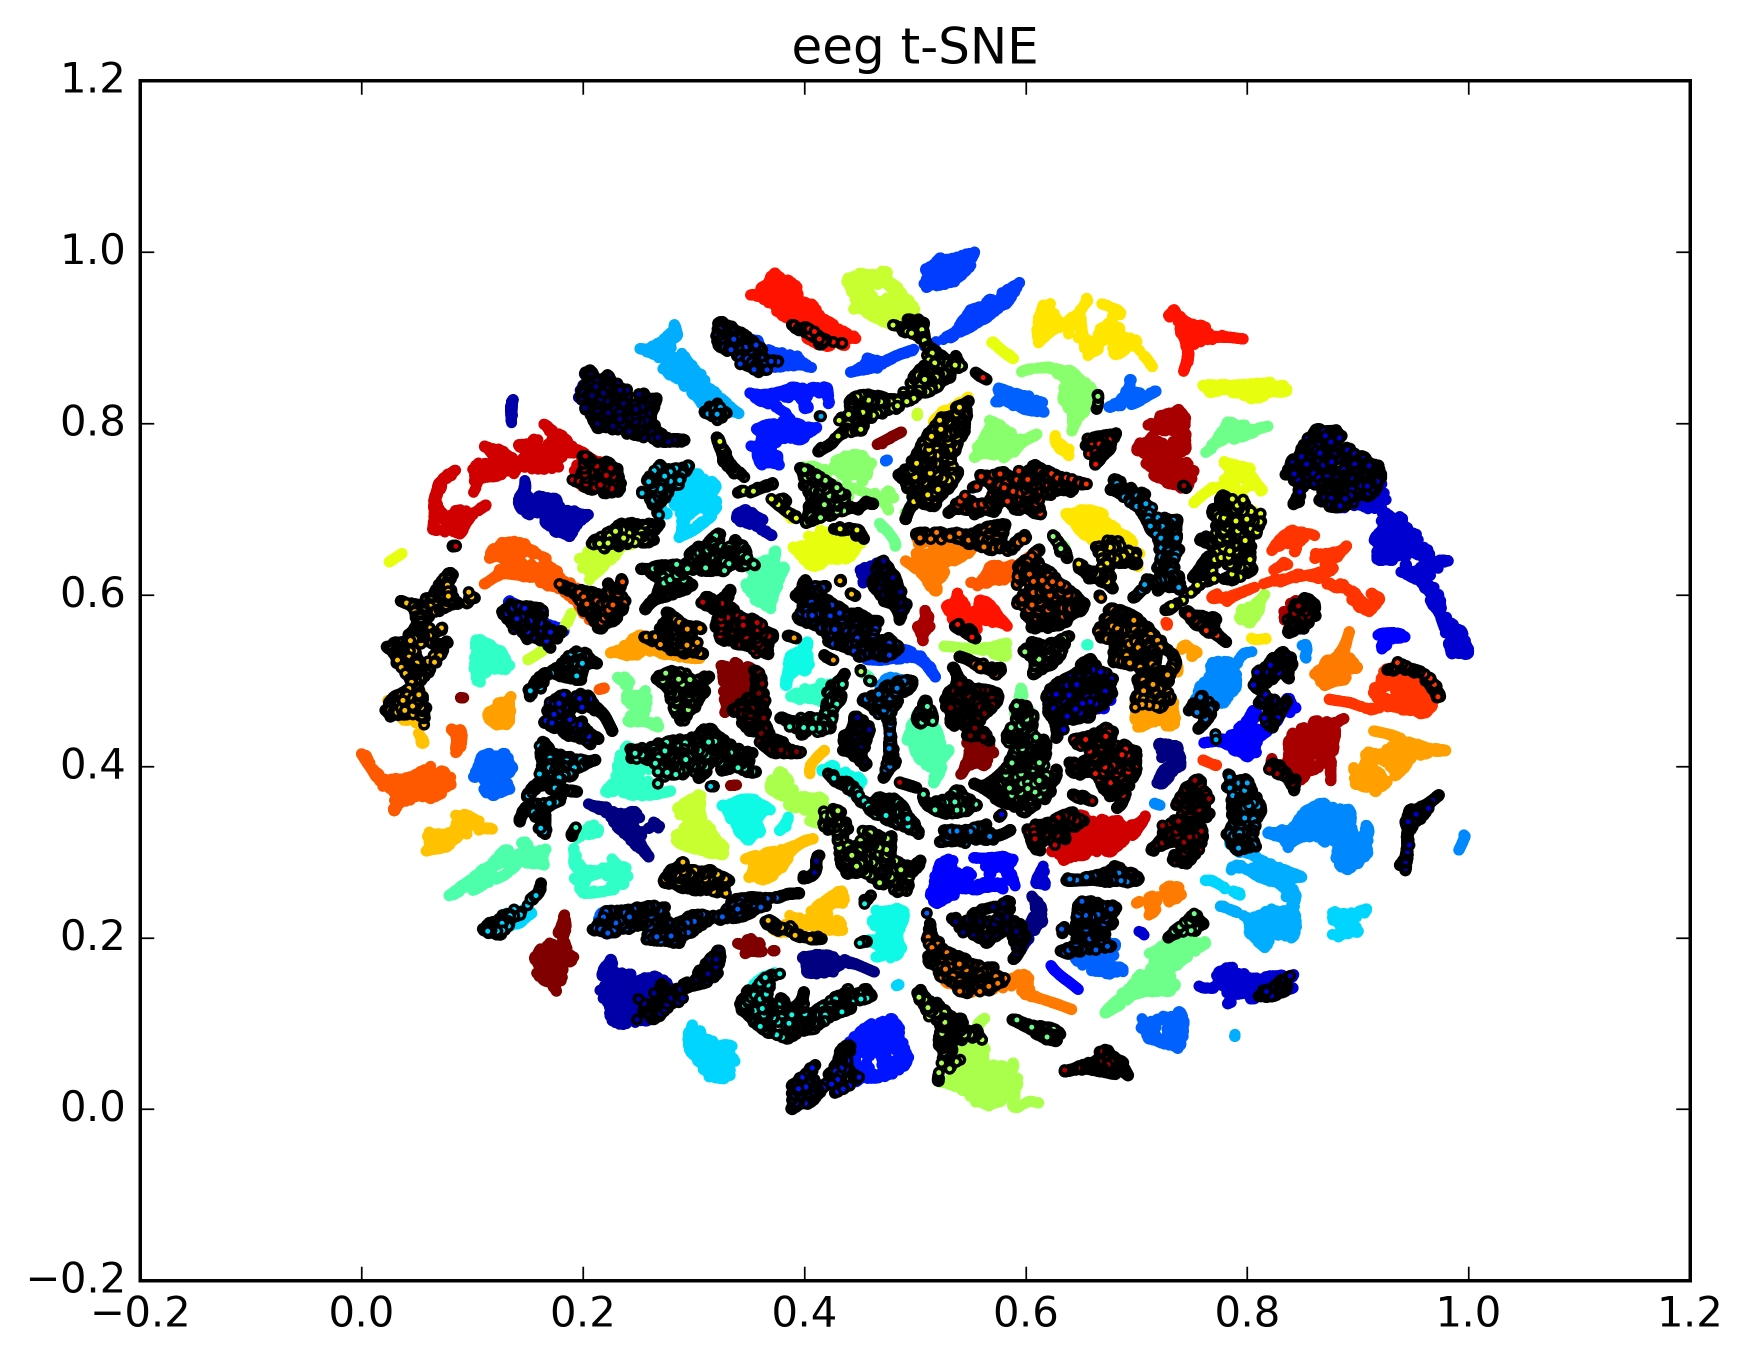
\includegraphics[width=3cm]{eegP6S3.jpg} & Participant 6, Series 3 & $0.04\%$ & Clearly separated data, which leads to extremely good performance on the neural net. \\ 
		\hline \rule{0pt}{15ex}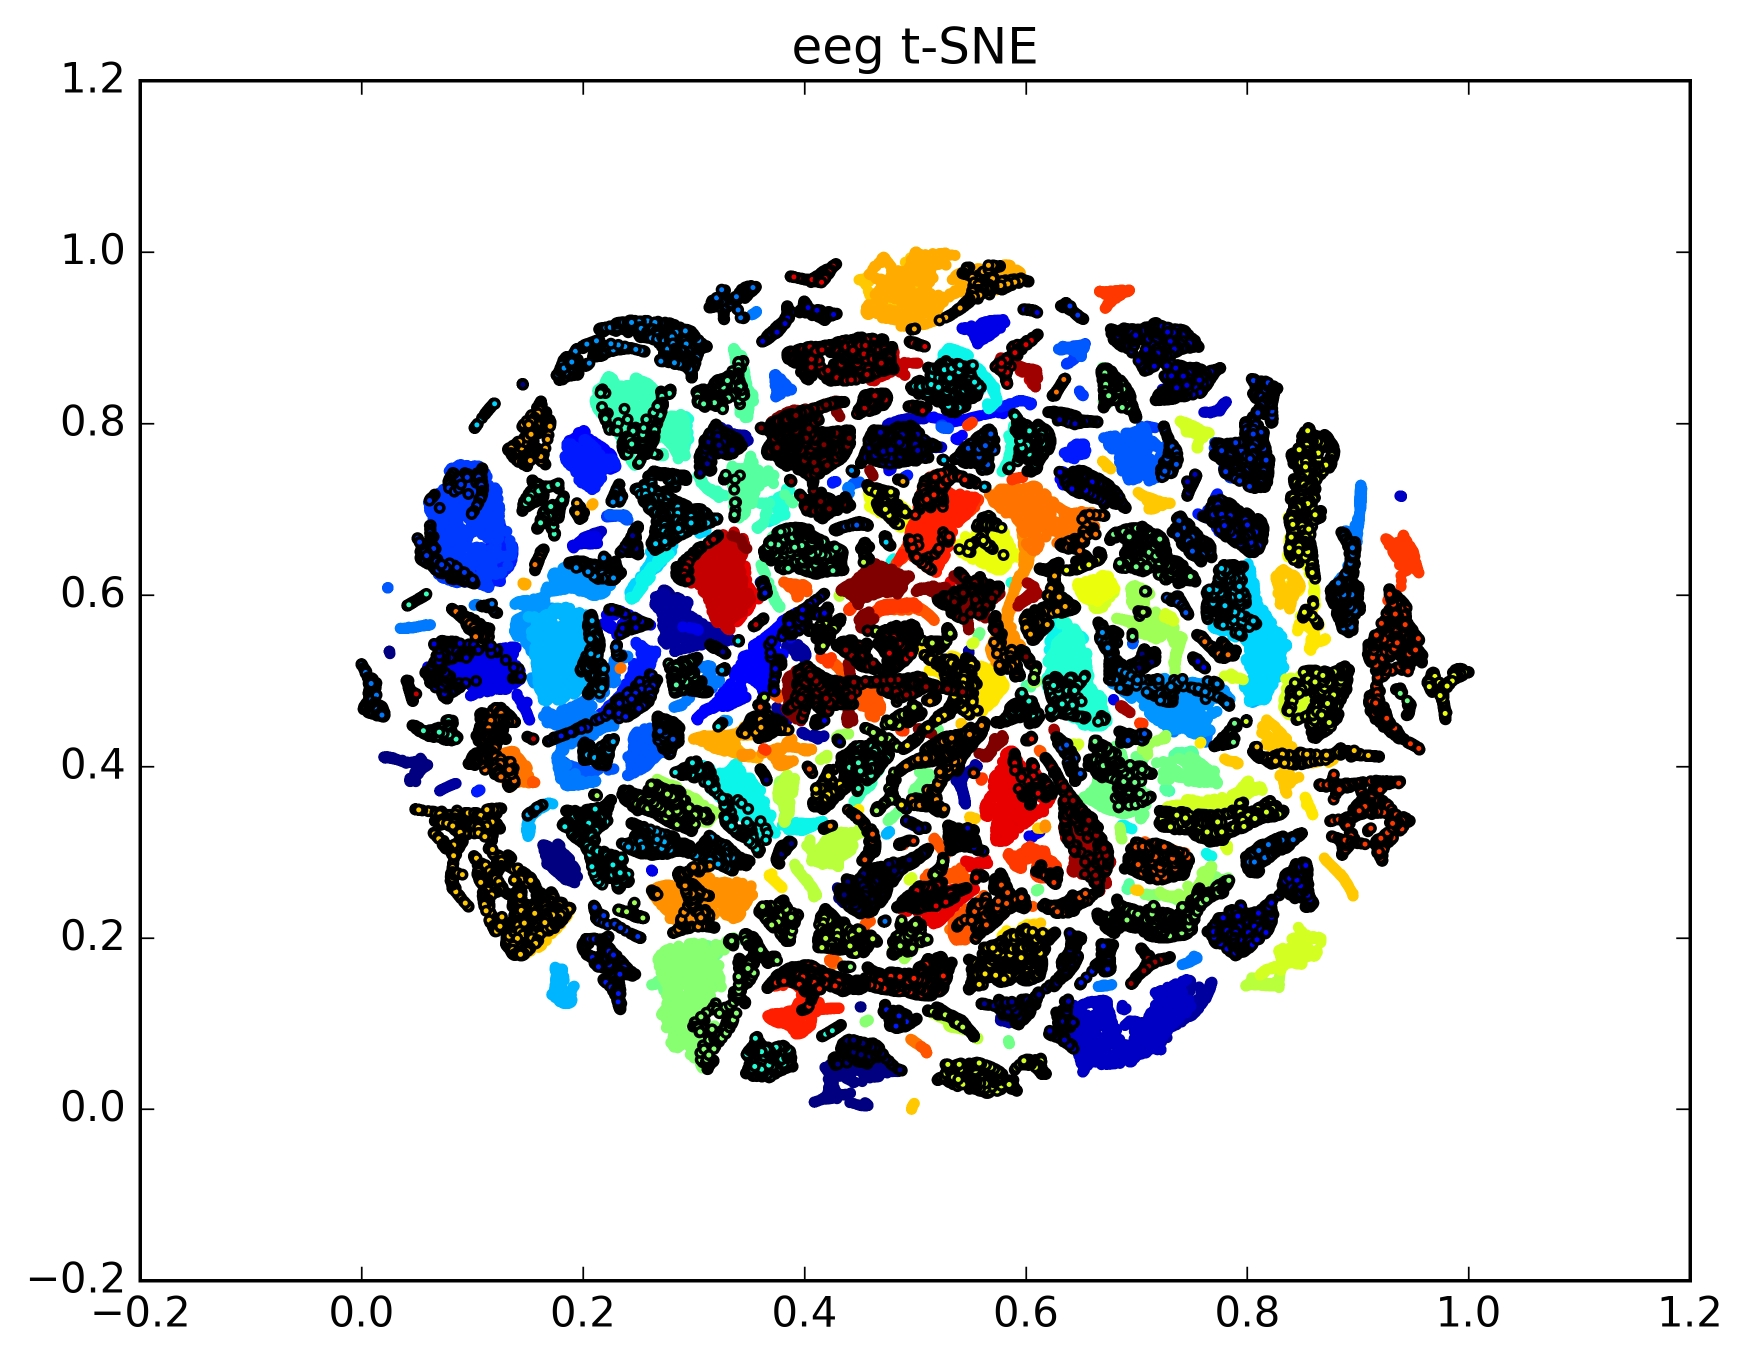
\includegraphics[width=3cm]{eegP7S8.jpg} & Participant 7, Series 8 & $29.99\%$ & Significantly more overlapping areas in the t-SNE plot. This is also reflected in the much worse error rate. \\ 
		\hline \rule{0pt}{15ex}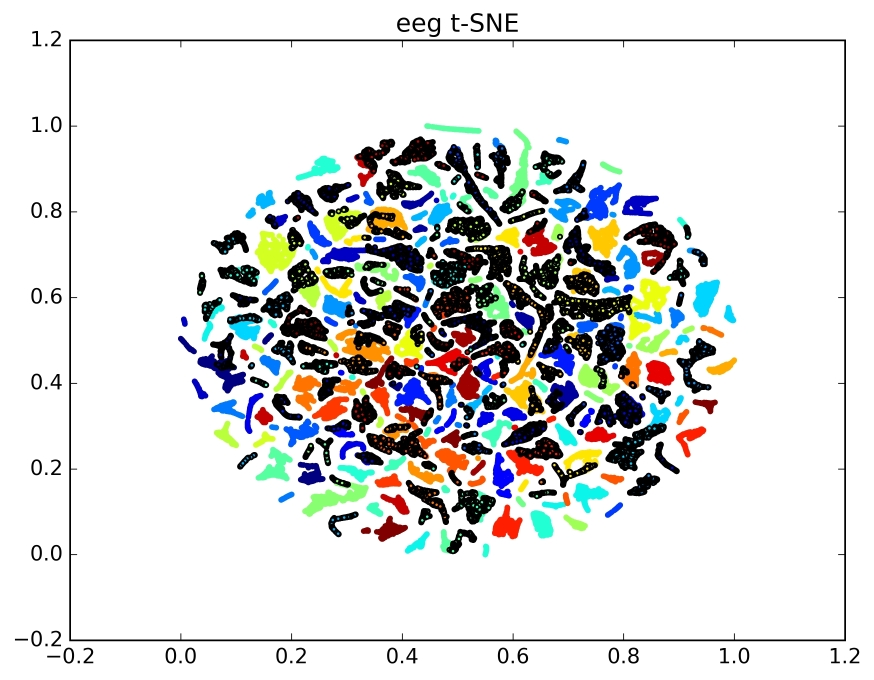
\includegraphics[width=3cm]{eegP9S5.jpg} & Participant 9, Series 5 & $0.03\%$ & Clearly separated data. Compared to other plots very many but small clusters are formed. The extreme error is again NOT a typo. \\  
		\hline \rule{0pt}{15ex}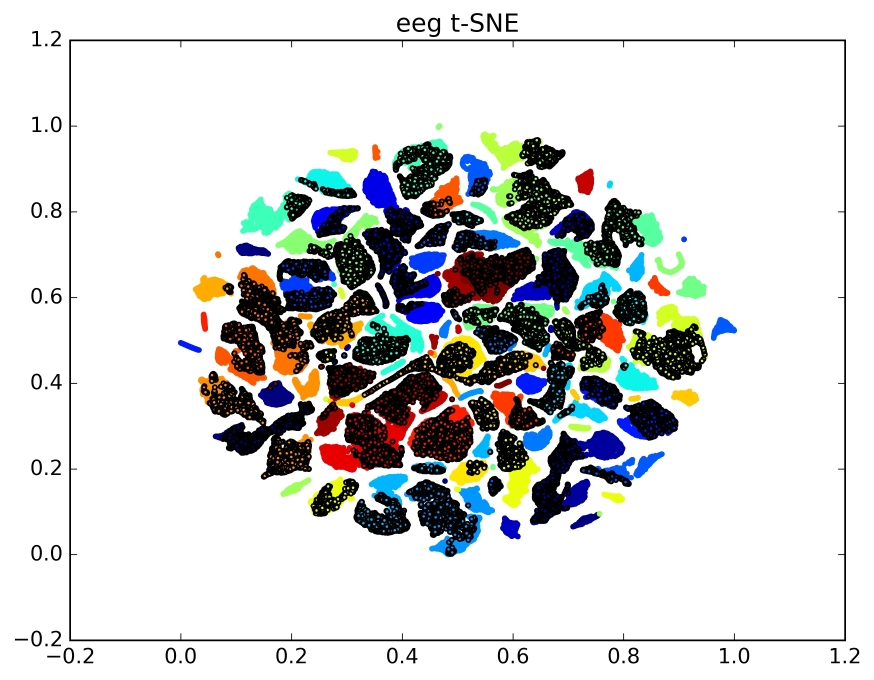
\includegraphics[width=3cm]{eegP12S2.jpg} & Participant 12, Series 2 & $0.11\%$ & Again clearly separated data and extreme error rate. \\ 
		\hline 
	\end{tabular}
	\label{tbl:tests}
	\caption{Running the same tests on various participants and series}
\end{figure}


\section{Conclusion}
Normalizing the datasets did not make any notable difference for participant 1, series 1. Running the same test on other participants and series revealed rather insane results. The trials of some of those sets could be classified basically perfectly. As these results are hard to believe, it is worth to mention once more that the correct function of both the t-SNE script as well as the neural net had been checked multiple times again using, inter alia, the reference datasets introduced in the previous paper.




\end{document}